\chapter{Curry--Howard对应} % (1934 -- 1969)
\section{简单类型\texorpdfstring{\(\lambda\)}{Lambda}-演算与命题逻辑}

经过上面的一些研究, 或许有些读者会产生一种模糊的感觉.
假如我们有 \(f : \alpha \to \beta\), 以及 \(a : \alpha\),
那么我们就能求值得到 \(f(a) : \beta\). 这其实和逻辑里
最古老的推理有些相像: 假如我们证明了 \(p\Rightarrow q\),
并且我们证明了 \(p\), 那么我们就可以证明 \(q\).

这是否能推广一下呢? 完全可以! \(p \wedge q\) 就对应了
Descartes 乘积 \(\alpha \times \beta\). 这个类型的
元素形如 \((a, b)\), 其中 \(a : \alpha, b : \beta\).
并且有两个投影函数 \(\pi_1(a, b) = a, \pi_2(a, b) = b\).
它们的类型写出来就是 \(\alpha \times\beta \to \alpha\)
以及 \(\alpha\times\beta \to \beta\). 对应到逻辑里面, \(\pi_1\)
恰好就是 “如果 \(p \wedge q\) 成立, 那么 \(p\) 成立”.

对偶地, \(p\vee q\) 则对应了类型的不交并, 记作
\(\alpha + \beta\). 它的元素要么形如 \(\iota_1(a)\),
要么形如 \(\iota_2(b)\). 而我们有一个函数对此分类讨论:
如果有 \(f : \alpha \to \gamma\) 与 \(g : \beta \to \gamma\)
分别处理两种情况, 那么
\[\cons{case}(f,g,c) = \begin{cases}
  f(a) & c = \iota_1(a)\\
  g(b) & c = \iota_2(b).
\end{cases}\]
而 \(\cons{case}\) 的类型就是
\((\alpha \to \gamma) \to (\beta \to \gamma)
\to (\alpha + \beta \to \gamma)\). (回忆我们之前
说的用 \(\alpha \to \beta\to \gamma\) 表示一个二元函数的技巧.)

我们总结一下上面的相似性, 可以发现可以把类型和命题做类比.
类型的元素就和命题的证明差不多, 因此命题的真假就可以解释为
对应的类型是否有元素. 我们可以定义一个类型 \(\mathbf 0\)
没有任何元素, 代表假命题. 则 \(\alpha \to \mathbf 0\)
代表命题的否定, 缩写成 \(\neg \alpha\). 我们对 \(\mathbf 0\)
的元素可以分类讨论, 但是由于只有零种情况, 因此得到
\[\cons{exfalso} : \mathbf 0 \to \gamma.\]
可以把这个与前面的 \(\cons{case}\) 对比. \(\cons{exfalso}\)
对应逻辑中的爆炸原理: 从假命题出发可以推出一切命题.

另一方面, (简单类型)组合子演算也有类似的现象. 这更加明显:
\(\cons{S}\) 的类型是 \((\alpha \to\beta\to\gamma)\to(\alpha\to\beta)\to(\alpha\to\gamma)\);
而 \(\cons{K}\) 则是 \(\alpha \to \beta \to \alpha\).
这刚好是 Hilbert 公理系统里面的两条公理! Curry 在
1934 年初步注意到组合子的这个性质\cite{curry:1934:combinatorCH}.
这个想法在后来几十年中逐步被推广. 人们发现, 用于计算、为数学对象
分类的类型, 与用于证明、只有真假的命题, 在许多方面上有着惊人的相似性:
\begin{itemize}
\item 组合子对应 Hilbert 命题逻辑演绎系统;
\item \(\lambda\)-演算对应自然演绎系统;\footnote{这是与 Hilbert 系统不同的另一个演绎系统.}
\item \(\lambda\)-演算可以转换成组合子, 对
应演绎定理.\footnote{演绎定理说的是,
如果假设 \(\varphi\) 成立, 在 Hilbert 系统中
可以证明 \(\psi\), 那么不需要任何假设就能在 Hilbert
系统中证明 \(\varphi \Rightarrow \psi\).}
\end{itemize}

我们或许可以大胆一些, 把这种相似性升格为\emph{同一性}:

\slogan{类型是命题.}

这就是 Curry--Howard 对应. 它体现了逻辑学和类型论
(进而与计算机科学) 有着深刻的内在联系.
需要注意的是, 之前介绍的简单类型论可以表达高阶逻辑, 但是
这个表达能力是额外加入的: 我们添加了命题的类型 \(o\),
并且加入了逻辑连词与公理. 但是在这里简单类型\(\lambda\)-演算
并没有加入任何关于逻辑的内容, 直接通过 Curry--Howard 对应
即可表达命题逻辑. 我们下面看看能从这之中挖掘出哪些有价值的数学.

\section{依值类型}

有了命题逻辑, 下一步自然是一阶逻辑, 或者称作谓词逻辑.
这里有形如 \(\forall x. P(x)\) 的命题. 直观上看,
它对应 “输入 \(x\), 输出 \(P(x)\) 对应的类型的元素”.
但是这有一点小问题: 对于不同的输入\emph{值}, 输出的%
\emph{类型}是不同的. 换句话说, 类型可以取决于值.
我们称陪域取决于输入值的函数为\textbf{依值函数}.

事实上, 这种函数我们在数学中早就见过了. 一个向量丛就是
给定流形上的点 \(x \in M\), 给出一个向量 \(\vec v \in \mathrm{T}_xM\)
的函数. 这里随着输入不同, 输出的向量所处的向量
空间也不同. 对于普通的集合也有这样的构造: 给定定义域 \(B\)
与一族集合 \(F_x, x \in B\), Descartes 乘积
\(\prod_{x\in B} F_x\) 就是一种依值函数.
对于 \(\exists x. P(x)\) 也是类似的. 它对应有序对
\((x, p)\), 使得 \(p \in P(x)\). 这对应集合的
不交并 \(\coprod_{x\in B} F_x\).

% TODO rewrite give more examples (...)

当然, 在通常数学中对依值函数的定义一般采取另一种方法.
考虑全空间 \(E = \coprod_{x:B} F_x\), 我们有一个
映射 \(\pi : E \to B\) 投影到 \(B\) 上. 依值函数
集合 \(\prod_{x:B} F_x\) 定义为
\[\{f : B \to E \mid \pi \circ f = \cons{id}\}.\]
这个定义在集合上和上面是等价的, 而在拓扑空间上这就是纤维丛的
截面. 推广到一般的数学对象上时, 也采用这个定义.

我们接下来会采用 \(\Pi, \Sigma\) 来指代这两种
类型. 它们的规则和函数、 Descartes乘积非常类似.
如果有变量 \(x : A\) 与表达式 \(M : B\), 其中
\(M, B\) 可以包含 \(x\) (注意在普通的函数类型定义
中, \(B\) 不得包含 \(x\)).
那么 \(\lambda x. M\) 的类型是 \(\prod_{x:A}B\).
反过来,
如果有表达式 \(N : A\), \(M : \prod_{x:A} B\),
那么 \(M(N)\) 的类型就是 \(B[x/N]\), 其中 \([x/N]\)
表示把变量 \(x\) 代入为 \(N\). 并且有 \((\lambda x.M)(N) = M[x/N]\).
读者可以自行写出 \(\Sigma\) 的规则. % TODO write this out
对于更详细的介绍, 读者可以参阅\cite{ufp:2013:hottbook}~的
第一章.

1967年, 利用这些想法, Nicolaas Govert de Bruijn
设计了一门依值类型论的计算机语言, 称为 Automath.
1976年, Jutting 在他的学位论文~\cite{automath:1994:automath}中使用 Automath
形式化了 Landau 的《分析学基础》. Automath 没有
被大规模使用, 不过它的设计影响到了许多后继的类型论.

F系统\footnote{这个名字是因为Girard的论文中用F
缩写法语单词\emph{ferm\'e} (闭), 阴差阳错成为了
现在普遍指代这个系统的名字.} (这严格来说不属于依值类型)
在 1972 年由逻辑学家 Jean-Yves Girard~\cite{girard:1972:systemf}
与 1974 年由计算机科学家 J. C. Reynolds~\cite{reynolds:1974:systemf} 独立发现.
一边是逻辑学, 一边是计算机科学, 这说明 Curry--Howard
对应不仅仅是一个巧合, 而是深刻地影响了两个学科的发展.

F 系统的规则对简单类型 \(\lambda\)-演算做了一点扩展.
它的类型除了函数类型 \(\alpha \to \beta\) 之外,
还有形如 \(\forall X. \beta\) 的类型, 其中
\(X\) 是类型变量, 表达式 \(\beta\) 可以
包含 \(X\). 这个类型表示 “不论 \(X\) 是什么,
都能充当 \(\beta\) 的元素” 的类型. 具体来说,
如果有一个可以包含 \(X\) 的表达式 \(M\),
对于任何类型 \(\alpha\), \(M[X/\alpha]\) 都是
\(\beta[X/\alpha]\) 类型的元素, 那么
\(\Lambda X. M\) 就是 \(\forall X. \beta\) 的元素.
而反过来, 如果 \(f\) 是 \(\Lambda X. M\) 的元素,
那么 \(f \alpha\) 就是 \(M[X/\alpha]\) 的元素.

举个例子, \(\Lambda X. \lambda x. x\)
就是 \(\forall X. X \to X\) 的元素. 在一些形式
中要求在 \(\lambda x\) 上标注出 \(x\) 的类型,
比如 \(\Lambda X. \lambda x^X. x\). 而在一些
形式中甚至不要求写出 \(\Lambda X\). 这些差别会对语言
的性质起到一定的影响, 但是我们这里不过多停留.

F系统包含很多奇特的构造. 比如我们可以像无类型
\(\lambda\)-演算中那样编码自然数. 定义类型
\(\mathbb N = \forall X. (X \to X) \to (X \to X)\),
那么之前构造的自然数 \(\lambda f. \lambda x. f(f(\dots(f(x))))\)
就可以在 F 系统里面写成
\(\Lambda X. \lambda f^{X\to X}. \lambda x^X. f(f(\dots(f(x))))\).
可以同样写出上面介绍过的加法、乘法、幂等等运算.
请读者思考为什么在简单类型 \(\lambda\)-演算中无法做到
这一点.

Girard 在他的论文~\cite{girard:1972:systemf}中
证明了二阶逻辑\footnote{这里其实移除了排中律, 下一节就
会提到相关内容.}中可以证明是全函数的递归函数\footnote{有一些
递归定义并不能产生处处有定义的函数, 比如 \(f(0) = 0,
f(n) = f(n-2)\), 这在奇数处就没有定义. 我们把处处有
定义的函数称为\textbf{全函数}.}在 F 系统中都能定义.
Reynolds 则从计算机科学的视角给出了一个反向的对应,
F 系统中能定义的 \(\mathbb N \to \mathbb N\) 的函数
都能在二阶逻辑中找到对应的逻辑关系. 这被称为
\textbf{Girard--Reynolds同构}.

F系统非常强大, 它可以构造很多类型. 譬如 \(\mathbf 1 =
\forall X. X \to X\), 可以证明它的唯一元素就是 \(\Lambda X. \lambda x. x\),
因此可以看作是单元素类型的定义. 而 \(\mathbf 2 =
\forall X. X \to X \to X\) 则恰好有两个元素 (请读者思考
是哪两个元素; 具体的证明则比较复杂, 需要语义工具).
上面我们构造了自然数类型, 这是递归类型的特殊情况.
F系统里面可以直接构造出大量的递归类型~\cite{wadler:1990:free}.
它甚至可以构造一个类型 \(V\),
使得 \(V\) 和 \((V \to \mathbf 2) \to \mathbf 2\) 同构.
这在集合的世界中是不可想象的: 一个集合永远比自己的幂集要
小, 更不用说自己的幂集的幂集了!
Reynolds~\cite{reynolds:1984:polymorphism}在1984年证明了
简单类型 \(\lambda\)-演算的集合论模型不能扩展到 F 系统.
因此, \ref{beginning:domain}~节中讨论的技巧在这里
构造语义就非常重要.

1988年, Coquand与Huet提出了构造演算 (Calculus of
Constructions, 缩写为 CoC). 这与上面提到的一些类型系统
很快被总结到同一个框架下, 统称为\textbf{纯类型系统}
(pure type system)~\cite{barendregt:1992:lambda}.
正常的依值函数类型的规则是
\[\frac{x{:}A \vdash B(x)\,\text{type}}{\prod_{x:A}B(x)\,\text{type}}\]
换句话说, 假设含有
变量 \(x : A\) 的表达式 \(B(x)\) 是合法的类型,
那么 \(\prod_{x:A}B(x)\) 也是合法的类型. 当然,
如果 \(B\) 不含变量 \(x\), 这就退化到普通的函数类型
\(A \to B\). 而F系统中的 \(\forall\) 类型只需要做
一点修改:
\[\frac{X{:} \blacksquare \vdash B(X)\,\text{type}}{\forall X. B(X)\,\text{type}}\]
但是这里 \(\blacksquare\) 中应该填入什么呢? 注意这里
\(X\) 是一个类型, 如 \(\forall X. X \to X\). 因此
我们需要一个符号表示\emph{类型的类型}. 即 \(X : \cons{type}\).
这样, 我们也不需要 \(A\,\text{type}\) 这样的声明,
而只需要 \(A : \cons{type}\) 就可以了. 那么F系统中的
规则就是
\[\frac{X{:}\cons{type} \vdash B(X):\cons{type}}{\forall X. B(X) : \cons{type}}.\]
我们甚至可以与上面依值函数类型的记号类比, 把 \(\forall X. B(X)\)
写成 \(\prod_{X : \cons{type}} B(X)\).

当然, 这立刻就会产生一个问题: \(\cons{type}\) 自己的类型
是什么呢? 在F系统里面, 由于 \(\forall X\) 中的 \(X\)
本身不能代入 \(\cons{type}\), 因此我们可以直接规定
\(\cons{type}\) 没有类型. 当然, 我们也可以引入一个
符号 \(\cons{kind}\), 满足 \(\cons{type} : \cons{kind}\).
这样因为上面的规则中要求 \(X : \cons{type}\),
所以 \(X\) 本身不能取值为 \(\cons{type}\). 这样我们的
改写仍然是等价的.

纯类型系统就是对这个观察的一个推广. 一般来说, 我们有
\[\frac{A : s_1 \quad x{:}A \vdash B(x) : s_2}{\prod_{x:A}B(x) : s_3}.\]
上面的依值函数就是 \((s_1,s_2,s_3) = (\cons{type}, \cons{type}, \cons{type})\)
的情况, 而 F 系统中的 \(\forall\) 则可以写成
\((s_1,s_2,s_3) = (\cons{kind}, \cons{type}, \cons{type})\)
的情况. 补上其他的规则, 我们可以总结出一个一般的定义.
\begin{definition}
\textbf{纯类型系统}是一族类型系统, 由三个参量决定:
一个集合 \(\mathcal S\),
其上有二元关系 \(\mathcal A\) 与
三元关系 \(\mathcal R\). 类型系统的规则有
\[\frac{}{\Gamma\vdash s_1 : s_2} \quad (s_1, s_2) \in \mathcal A\]
对于每组\((s_1,s_2,s_3)\in \mathcal R\),
类型系统中都添加两条规则:
\[\frac{\Gamma \vdash A : s_1 \quad \Gamma, x{:}A \vdash B(x) : s_2}{\Gamma \vdash \prod_{x:A} B(x) : s_3}\]
\[\frac{\Gamma \vdash A : s_1 \quad \Gamma, x{:}A \vdash B(x) : s_2\quad
\Gamma, x{:}A \vdash F(x) : B(x)}
{\Gamma \vdash \lambda x. F(x) : \prod_{x:A}B(x)}.\]
如果条目 \(x : A\) 在列表 \(\Gamma\) 中出现, 则有
\[\frac{}{\Gamma \vdash x : A}.\]
最后有
\[\frac{\Gamma \vdash F : \prod_{x:A}B(x) \quad
\Gamma \vdash M : A}{\Gamma \vdash FM : B(A)}\]
这里严格来说应该写成 \(B[x/A]\).
\end{definition}
在上面的例子中 \(\mathcal S = \{\cons{type}, \cons{kind}\}\),
\(\mathcal A = \{(\cons{type}, \cons{kind})\}\).

这里有一个非常重要的问题需要注意: 既然类型中可以包含
普通的值, 譬如 \(P(n)\) 表示 \(n\) 维的向量的类型,
那么如果我有一个向量 \(v : P(1+1)\), 是否可以说
\(v : P(2)\) 呢? 我们当然需要允许这样的推断, 否则
依值类型的意义就不大了. 因此我们需要修改上面类型系统的定义,
加入一条规则:
\[\frac{\Gamma \vdash M : A \quad A = B}{\Gamma \vdash M : B}\]
这里的等号与上面说的一样, 实际上是在表达式上定义的一个等价
关系, 如 \((\lambda x. x)y\) 与 \(y\) 等价.
在定义更加复杂的类型论时, 我们经常会发现这个等价关系附带上
类型信息会更加方便. 换句话说, 我们对于每对 \(\Gamma, T\),
在所有满足\(\Gamma \vdash A : T\) 的表达
式 \(A\) 构成的集合 \(U_{\Gamma, T}\) 上各自定义一个
等价关系, 而不是在全集 \(\bigcup_{\Gamma, T} U_{\Gamma, T}\) 上定义.
技术上的细节可以参考~\cite{barendregt:1992:lambda}.

如果我们设 \(\cons{type} : \cons{type}\) 会如何呢?
换句话说, 我们试图让 \((\cons{type}, \cons{type}) \in \mathcal A\).
结果或许并不令人意外: Russell悖论重新回到了类型论中!
因此我们不能设定存在所有类型的类型, \(\cons{type}\) 自身
的类型必须是别的东西. 然而, 即使 \(\mathcal A\) 中没有
这样的循环, 我们仍然可以导出矛盾. 1972年, Girard构造出了
U系统.
这个系统中 \(\mathcal S\) 有三个元素,
\(\cons{type}, \cons{kind}, \cons{Kind}\).
\(\mathcal A = \{(\cons{type}, \cons{kind}), (\cons{kind}, \cons{Kind})\}\).
也就是说这里只有 \(\cons{type} : \cons{kind} : \cons{Kind}\),
没有循环. 然而, 这个系统中仍然能够构造出类似的悖论, 我们称为
Girard悖论. 因此, 设计纯类型系统时必须小心.

\textbf{构造演算}中, \(\mathcal S = \{\cons{type}, \cons{kind}\}\),
并且 \(\cons{type} : \cons{kind}\). 而
\[\mathcal R = \{(s_1,s_2,s_2) \mid s_1, s_2 \in \mathcal S\}.\]
因此构造演算包含了普通的依值函数类型与F系统中的\(\forall\)类型,
还包含了两种新的依值函数类型. 这个系统已经证明是没有类似的悖论的.
事实上它有很好的典范性. 它包含了F系统, 所以自然地携带了
F系统中强大的编码能力, 如可以直接使用\(\forall\)类型定义
自然数类型, 等等. 因为继续扩展这个系统很容易导致 Girard 悖论
出现, 构造演算以及其各种子系统成为了纯类型系统中应用最广泛的系统.

\section{经典逻辑}

前面我们提到简单类型 \(\lambda\)-演算与命题逻辑之间
有对应关系, 称作Curry--Howard对应. 实际上, 这个对应
并不完美, 唯一的差异就在于排中律: 对于任何命题 \(p\),
\(p \vee \neg p\) 都是真命题. 注意这和矛盾律的区别:
对于任何命题 \(p\), \(p \wedge \neg p\) 都是假命题.
当然, 我们仍然可以证明 \(\neg \neg (p \vee \neg p)\),
但是我们不能消去双重否定.\footnote{注意这和
\(\neg\neg (\forall p. p \vee \neg p)\) 不同,
我们无法证明这个命题.}

为什么简单类型 \(\lambda\)-演算无法推出排中律呢? 我们
可以看一个模型. 给定一个拓扑空间 \(X\), 其上的开集代表
命题, 并集代表 \(p \vee q\), 交集代表 \(p \wedge q\).
而\(\neg p\) 被表示为 \(p\) 的补集\emph{的内部},
\(p \to q\) 被表示为 \((X \setminus p) \cup q\) 的内部,
全集和空集分别代表真命题和假命题. 一条逻辑规则
\(\frac{p_1~p_2 \cdots}{q}\) 表示 \(p_1 \cap p_2 \cap\cdots\) 包含 \(q\).
读者可以验证发现这满足所有的逻辑规则, 但是对于排中律来说,
某个开集并上它补集的内部并不一定是全集. 由此看来, 排中律的
缺失实际上有一些几何的内涵. 我们之后会进一步探究几何上的
联系.

我们还有另一种方法. 在简单类型 \(\lambda\)-演算中, 可以证明
不含自由变量的类型为 \(\alpha + \beta\) 的元素,
必然等价于形如 \(\iota_i(M)\) 的表达式. 这也就是说,
在简单类型 \(\lambda\)-演算中, 没有其他条件的情况下
证明命题 \(p\vee q\), 就必须要确定地构造出具体哪一边是成立的.
而排中律 \(p \vee \neg p\) 自然不能直接确定哪一边成立,
因此是无法证明的. 上面这两种方法, 前者是通过观察语义,
而后者是通过直接分析语法.

我们在 \ref{ch:classical}~节会讨论如何在类型论的
Curry--Howard 对应中加入排中律. 但是
我们首先不妨来看看缺少排中律
会引发什么变化. 我们将含有排中律的逻辑
称作\textbf{经典逻辑}.\footnote{经典逻辑的不少定义中,
排中律是作为其它规则的推论存在的,
正如Zorn引理一般是作为选择公理的推论存在的. 因此在这些定义
下无法谈论直接“去掉”排中律. 因为我们不会涉及定义的细节,
这里不讨论具体如何从形式系统中去掉排中律.}
\begin{theorem}
排中律有如下的等价形式.
\begin{itemize}
\item 排中律: \(p \vee \neg p\).
\item 双重否定消去: \(\neg\neg p \to p\).
\item 逆否命题: \(\neg p \to \neg q\) 等价于 \(q \to p\).
\item Peirce定律: \(((p \to q) \to p) \to p\).
\item Peirce定律的特殊情况: \((\neg p\to p) \to p\).
\end{itemize}
\end{theorem}
\begin{theorem}[Diaconescu]\label{ch:diaconescu}
选择公理可以推出排中律.
事实上排中律可以表述为“\(\{0,1\}\)满足
选择公理”.\footnote{集合\(Y\)满足选择公理, 当且仅当
对于任何集合 \(X\) 与关系 \(R \subseteq X \times Y\), 如果对于
任何 \(X\) 的元素 \(x\) 都存在 \(Y\) 的元素 \(y\)
满足 \(xRy\), 那么存在一个函数 \(f : X \to Y\) 使得
\(xRf(x)\). 完整的选择公理说的就是所有集合都满足选择公理.}
\end{theorem}

一个最经典的使用排中律的证明是这样的.
\begin{theorem}
存在无理数 \(a,b\) 使得 \(a^b\) 是有理数.
\end{theorem}
\begin{proof}
考虑 \({\sqrt2}^{\sqrt2}\). 它要么是有理数要么是无理数.
如果是前者, 则命题成立. 如果是后者, 设 \(a = {\sqrt2}^{\sqrt2},
b = \sqrt 2\), 则
\[a^b = \left({\sqrt2}^{\sqrt2}\right)^{\sqrt2} = {\sqrt2}^{\sqrt2\times\sqrt2} = 2.\]
因此无论 \({\sqrt2}^{\sqrt2}\) 是有理数还是无理数,
都存在 \(a^b\) 满足条件.
\end{proof}
\begin{remark}
一个不使用排中律的方法是考虑 \(a = \sqrt 2, b = \log_2(9)\).
另一个避免排中律的方法是花费功夫证明 \({\sqrt2}^{\sqrt2}\) 确实
是无理数, 这需要非常复杂的数论证明.
\end{remark}

那么正常的数学研究中多大程度上需要排中律呢? 实际上直到
Hilbert之前的绝大部分数学研究都完全可以绕过排中律.
Hilbert之后的数学也可以发展无需排中律的版本.
现在已经有不少不使用排中律发展数学的努力,
包括代数、几何、分析等等. 在没有排中律时,
会出现很多有趣的现象: 很多数学概念
会分裂成多个不等价的概念 (实际上会分裂出无数个不同的概念, 但是
正如正常数学中我们一般只会取有意义的概念研究, 在这里我们
也只会谈比较重要的版本). 譬如域在没有排中律的时候会出现%
\emph{离散域}与\emph{连续域}的变体, 有理数
\(\mathbb Q\) 是离散域, 而
实数 \(\mathbb R\) 则是连续域. 注意这里完全没有
涉及任何拓扑信息! 在有排中律时, 离散域与连续域都等价于
通常的域的定义, 这样这个非常有意思的区分就被抹平了.

另一方面, 事实上去掉排中律完全没有使得能够发展的数学受到限制,
恰好相反, 去掉排中律使得数学变得更丰富了. 这是因为
对于任何一个命题 \(p\), 都存在一个命题 \(p^{\cons{N}}\),
使得这个命题在无排中律下 \(p^{\cons{N}}\) 可证当且仅当
\(p\) 在使用排中律时可证, 并且在有排中律时 \(p^{\cons{N}}\)
与 \(p\) 等价. 例如 \(\forall x. p(x) \vee q(x)\)
会被翻译为 \(\neg \neg \forall x. \neg (\neg p(x) \wedge \neg q(x))\).
因此无排中律时的数学严格包含了
有排中律时的数学. 换个说法, 排中律使得大量原先不等价的
命题变得等价, 所以不加入排中律会让数学更加丰富, 同时不会
有任何损失. Hilbert 说过:“将数学家的排中律夺走, 就好比
禁止拳击手使用拳头.” 在这个意义下, 这句话自然是不正确的.

仅仅是去掉排中律, 得到的是\textbf{中性数学}. 因为排中律
仅仅是不可证明或证伪, 中性数学中随时可以重新加入排中律.
反过来说, 这留出了额外的空间, 让我们可以加入\emph{与排中律相
矛盾的公理}. 即加入一些公理使得 \(\neg (\forall p. p \vee \neg p)\)
成立. 例如我们可以加入“所有函数 \(\mathbb R \to \mathbb R\)
都是连续函数”. 这样的公理被称为\textbf{反经典}的.

\subsection{构造主义}

前一节中已经提示了, 在没有排中律时, 任何数学对象都必须
构造出来才可以认为存在. \(p \vee q\) 的证明必须明确
给出哪一边成立, 而 \(\exists x. p(x)\) 必须具体给出
一个 \(x\). 因此, 我们将这种逻辑以及相关的各类数学哲学
思想称为\textbf{构造主义}. 如果读者对放弃排中律仍然有怀疑,
可以阅读《接受构造主义的五个阶段》\cite{bauer:2016:fivestage}.
这篇简短的文章借用了心理学上人们接受悲痛与失去的
五个阶段 ------ 否认、愤怒、恳求、沮丧、接受 ------ 来
探讨对构造主义的一些常见误解, 以及构造主义对数学的贡献.
下面的介绍主要参考了~\cites{carl:1998:brouwer}{sep:2022:constructive}.

\subsubsection{直觉主义}

在19世纪, 数学家逐渐开始将许多过去定义模糊的概念
严格化. 我们发现可以将实数定义为有理数的Cauchy列.
Cantor的工作为无穷数列、无穷集合等等概念夯实了基础,
并且区分了仅仅是稠密的集合(如有理数)与真正的实数连续统.
Frege将自然数也使用集合做了定义 ------ 自然数\(n\)
就是所有恰好有\(n\)个元素的集合构成的集合; 自然数集
\(\mathbb N\) 就是所有有限集在双射下构成的等价类的集合.
Kronecker与Poincar\'e等数学家在19世纪末期对此
提出了质疑. 他们认为这些使用无穷集合, 并且在许多情况下
都是非构造性质的概念是无法作为数学的根基的.

在世纪之交, Russell悖论的发现动摇了这套基础.
(我们最终因为这个原因抛弃了Frege对自然数的定义,
但是Cauchy列, Cantor的连续统等等概念仍然保留了下来.)
Hilbert为了应对这次危机, 提出了一套纲领. Hilbert
认为我们可以信任有限的算数与组合, 希望能给出
一套描述无限集合的公理系统, 并且用纯有限的方法证明这套
公理系统的自洽性. 这样就可以将无限的概念从数学危机
中拯救出来. Hilbert认为, 我们可以将关于无限的数学
化归为对命题机械地按照形式系统的规则操作的过程.

我们现在知道, 以G\"odel的不完备性定理为代表的对
形式系统更进一步的研究粉碎了Hilbert原本的愿望, 不过
在当时这还并未明晰. Brouwer 继承了 Kronecker 的思想,
对Hilbert纲领发起了抨击. 关于Brouwer与Hilbert的论争
的历史, 读者可以参阅~\cite{carl:1998:brouwer}.
Brouwer认为, 数学是人类的精神活动.
数学思想先于语言而存在, 仅仅对命题进行机械操作
是不可能完全囊括数学的全部内涵的. 这些数学哲学观点
就是\textbf{直觉主义}. 遵循这些思想, Brouwer构建了
一套直觉主义数学基础.

直觉主义作为构造主义的一个分支, 拒绝排中律无限制的使用.
Brouwer认为, 只有关于有限个事物的命题, 才能使用排中律
------ 因为对于有限个事物我们可以逐一检查命题是否成立.
我们不能随意地推广到无限的集合. 譬如考虑命题 \(p\):
“对于所有偶数 \(n \ge 4\), \(n\) 可以表示为两个质数的和”.
并没有理由认为 \(p \vee \neg p\) 成立, 因为
不可能在有限的时间内穷尽所有的偶数. 我们将来可能会给出
一个无法被表示为两个质数之和的偶数; 也有可能得到一个算法,
保证任意给定一个偶数都能找出对应的两个质数. 但是在那一刻
到来之前, 我们不能从对有限集合的经验出发, 直接认为这两者
之一一定成立.

不过, 直觉主义数学并不严格要求一切数学对象都需要被完全
确定地构造出来.
\begin{quotation}
允许两种创造数学对象的方法: 第一种是无穷序列, 每一个元素
都可以从已经得到的数学对象中自由选择[...]; 第二种是集合,
之前构造出的数学对象中, 满足某个性质的所有对象构成一个集合,
前提是如果一个对象满足该性质, 那么
与这个对象按照定义“相等”的其他对象也满足该性质.~\cite{brouwer:1981:intuitionism}
\end{quotation}
在其他风格的构造主义中, 对于一个无限数列通常要求存在
一个算法能够给定 \(n\), 计算出这个数列的第 \(n\) 项.
但是 Brouwer 的直觉主义中允许所谓的\emph{自由选择序列},
即不需要确定的算法, 可以自由选择. 利用这些自由选择序列,
Brouwer构造出了直觉主义的实数集.

拒绝排中律使得实数集表现得更像延绵连续的整体. 在经典数学中,
实数集是“脆”的, 因为可以随时定义不连续的函数:
\[f(x) = \begin{cases}
1 & (x > 0)\\
0 & (x \le 0).
\end{cases}\]
经典数学中必须在实数集的基础上定义拓扑, 才能将
连续性这样直观的概念恢复出来. 由于没有排中律, 直觉主义的
实数并不能证明 \((x < 0) \vee (x = 0) \vee (x > 0)\)
一定成立, 因此无法随意地分割实数. Brouwer 采用了更加
适合构造主义的\textbf{分离性}(apartness), 即定义一个
关系 \(x \mathop{\#} y\) 为“存在 \(\epsilon > 0\)
使得 \(|x - y| > \epsilon\)”. 在经典数学中, 这与
\(x \ne y\) 等价, 但是在构造主义数学中这给出了具体的 \(\epsilon\) 的
构造, 因此比 \(x \ne y\) 更强. 譬如可以证明任何
实数 \(x \mathop{\#} 0\) 都有倒数, 但是将条件换为
\(x \ne 0\) 就无法证明.

由直觉主义的数学哲学出发, Brouwer进一步提出了一些公理.
从这些公理出发, 直觉主义脱离了仅仅是移除排中律的中性数学
的范畴, 而是与经典逻辑中的结论相矛盾, 对实数连续统建立
起了迥然不同的理论体系. 例如
著名的一致连续性定理:
\begin{theorem}[Brouwer]
给定度量空间 \(X,Y\), 其中 \(X\) 完备并且完全有界.
则任何映射 \(X\to Y\) 都是一致连续的.
\end{theorem}
\begin{corollary}\label{ch:brouwer:funny}
任何函数 \(f : [0,1] \to [0,1]\) 都是一致连续函数.
\end{corollary}
但是需要注意的是, 此时
可以认为Brouwer的实数已经与经典数学中的实数不是同一个概念了,
因此不能简单的说直觉主义数学与经典数学是“互斥”或者“矛盾”的.
它们仅仅是在命题的形式上有表面的互斥关系, 而实际情况需要
对各自的数学哲学进行更细致的解读.

1930年, Brouwer 的学生 Arend Heyting 提出了一套形式逻辑系统,
试图刻画直觉主义中使用的逻辑. 这套形式系统大致就是一阶逻辑
去掉排中律. 因此, 许多文献中也用\textbf{直觉主义逻辑}一词
来指代去掉排中律的逻辑. 我们前文中已经提到, 这类
逻辑更准确的名字是中性逻辑.

\subsubsection{俄罗斯构造主义}

在1940年代末, 俄罗斯数学家 Andrey A. Markov
({\tempfont Андре́й Андре́евич Ма́рков}, 与他的父亲同名; 他的父亲
是提出Markov链的人) 构建了构造主义逻辑的另一个
分支 ------ 俄罗斯构造主义, 也称作递归构造主义.
在这个流派中, 一切数学对象都使用适当的递归函数构造.

递归函数的概念在1933年由G\"odel与Jacques Herbrand在
研究形式系统的性质时提出, 是一类特殊的自然数上的
多元函数 \(\mathbb N^n \to \mathbb N\);
在1936年Church的(无类型) \(\lambda\)-演算中, 使用 \ref{beginning:lambda}~节
中提到的编码自然数的方式, 也可以考虑能够在 \(\lambda\)-演算
中写出来的自然数上的多元函数; 同年, Alan Turing 试图
刻画“存在有效的方法计算”的概念时, 提出了 Turing 机. 令人惊讶的是,
这三者给出的是等价的定义. 我们现在将这些定义统称
为\textbf{可计算函数}或者\textbf{一般递归函数}.
如输入自然数 \(n\), 输出第 \(n\) 个质数的函数,
就是一个可计算函数.\footnote{不可计算的函数反而在一般数学
中比较少见, 其中一个例子是将所有的命题用自然数做(合理的)编号,
对于编号 \(n\) 的命题, 如果它在ZFC公理系统下可以证明,
那么定义函数 \(f(n) = 1\); 否则定义 \(f(n) = 0\).
这种命题的编号称作 \textbf{G\"odel 编码}.}

一般递归函数对某些输入可能会无限地计算下去, 如定义
\[f(n) = \begin{cases}
f\left(\left\lceil \frac n2 \right\rceil\right) & (n \ge 1)\\
0 & (n = 0).
\end{cases}\]
那么计算 \(f(1)\) 时就会无限递归下去. 此时我们认为
\(f(1)\) 是未定义的. 如果某个函数对一些输入是未定义的,
我们则称其为\textbf{部分函数}. 除法就是我们最熟悉的部分函数,
它对除以零的情况没有定义. 对所有输入都有定义的函数
称为\textbf{全函数}. 在讨论可计算函数时, 除非额外强调,
“函数”一词通常指代部分函数.

递归函数就是那些能通过明确的方法计算的函数, 符合构造主义的
大致方向. 需要注意的是, 算法都是有限长的, 因此
能够写出的算法只有可数个, 所以 \(\mathbb N \to \mathbb N\)
的可计算函数也只有可数个.
在俄罗斯构造主义中定义的实数, 对应着经典数学中的\textbf{可计算实数}.
尽管可计算实数只有可数个, 但是我们遇到的绝大部分实数都是
可计算的, 如 \(\pi, e, \tan\sqrt{114514}\), 等等.
这使得构造主义中很多看似离奇的命题有了合理的解释: 将实数
改为为可计算实数, 函数改为为可计算函数, 以此类推, 这样得到的
命题在经典数学中也合理了起来.

\subsubsection{Bishop构造主义}\label{ch:bishop}

然而, 上面提到的构造主义流派在一段时间内都没有产出
其他数学家看来有重大意义的成果. 同时, 有很多类似
推论~\ref{ch:brouwer:funny} 的, 看起来完全是
稀奇古怪或者自相矛盾的结论.
在当时看来, Hilbert 所评价的 “将数学家的排中律夺走,
就好比禁止拳击手使用拳头” 确实显得有些道理.
在1967年, Errett Bishop 出版了一本构造主义分析学的书.
\begin{quotation}
Bishop的工作的意义在于证明了原本Hilbert与Brouwer都同意
的一个重要观点是错误的. 两人都认为, 如果真的要发展构造主义数学,
那么就必须 “放弃” 许多现代数学中关键的部分(例如测度论或者复分析).
Bishop展示了这完全是错误的. [...] 只不过我们需要选择
使用一种优雅的方式进行研究, 而不是用Hilbert所谓
的“拳击手的拳头”.~\cite{beeson:1985:constructive}
\end{quotation}

Bishop认为, 要构造一个集合, 只需要说明如何构造它的元素,
并且说明构造出的两个元素如何判断相等. 这种定义集合的方式
现在被称为 \textbf{Bishop 集合}. 在现代
类型论\footnote{Bishop并没有使用类型论, 这是后人的工作.}的语境下,
这就是一个类型上配备了一个等价关系, 称作\textbf{广集} (setoid).
我们可以紧接着将“广集函数”定义为尊重这个等价关系的函数.
换句话说, 给定广集 \((A, \sim_A),(B, \sim_B)\),
要构造广集 \(A \Rightarrow B\)的元素, 只需要给出一个
对应法则 \(f : A \to B\), 使得 \(x \sim_A y\) 时
\(f(x) \sim_B f(y)\). 给定两个这样的元素 \(f,g\),
我们要说明如何判断它们相等, 也即定义等价关系
\(f \sim_{A\Rightarrow B} g\). 为此, 我们规定
\[(f \sim_{A\Rightarrow B} g) \iff \forall x, f(x) \sim_B g(x).\]
读者可以验证这确实是等价关系.

Bishop用行动展示了数学的许多重要的部分都能在构造主义中发展,
并且只需要对经典数学的理论做较小的修改. 正如前面的引文所说,
我们只需要选取一种优雅的姿态, 就能在构造主义中轻松地完成
经典数学中可以做到的事情. 行胜于言, Bishop极大地推动了
构造主义数学的发展.

\subsubsection{Martin-L\"of构造主义}
1970年代, Martin-L\"of提出了一种构造主义的类型论,
我们现在称作\textbf{构造主义类型论}或者\textbf{Martin-L\"of 类型论}
(Martin-L\"of type theory, 缩写为MLTT).
我们会留出一章专门讲述, 这里按下不表. 从 Martin-L\"of 的
理论开始, 构造主义与类型论变得密不可分. 不过需要提醒读者,
类型论在Russell起初提出时, 完全是经典逻辑的. 所以说
尽管类型论与构造主义有很强的关联, 但是并没有包含关系.

\subsubsection{构造主义的几何意义}
\begin{figure}[ht]
\centering
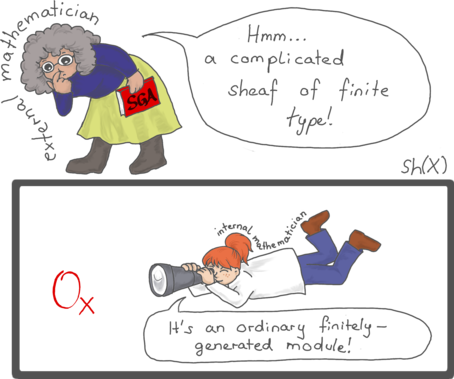
\includegraphics[width=0.5\textwidth]{images/external-internal-small.png}
\end{figure}
在当代的几何研究中, 构造主义又被赋予了新的内涵.
一些复杂的几何对象与简单的代数结构在操作上
有相似之处, 例如有限型的模层(sheaf of modules of finite type)是
非常复杂的对象, 而它对应的就是有限生成模.

我们可以使用这种相似的对应关系大大简化一些证明.
但是仔细考察这个对应关系, 会发现排中律没有对应.
几何学家可以选择在经典逻辑中写下繁琐且难以阅读的证明,
或者选择在一种构造主义的语言中写出简洁的证明. 这种
语言是\textbf{内语言}, 我们会在 \ref{category:inner}~节
介绍. 注意这并不是说放弃了排中律. 即使我们认为排中律成立,
这也仅仅是在外部成立, 而在外部进行证明时, 我们就要处理
譬如“有限型的模层”等概念. 在内语言中, 我们只需要处理
有限生成模, 而代价是不能使用排中律. 在内语言中写下的证明,
都可以翻译成外部语言中对复杂几何对象的操作. 有代数几何
基础的读者可以参阅~\cite{blechschmidt:2021:internal}.
插图取自\href{https://github.com/iblech/internal-methods}{此处},
这里也含有\cite{blechschmidt:2021:internal}的一份
副本, 以及许多相关的讲座幻灯片.

\subsection{经典逻辑的Curry--Howard对应}\label{ch:classical}

除了研究不含排中律的逻辑之外, 另一个方向自然的问题就是
经典逻辑是否有 Curry--Howard 对应. 答案是肯定的.
首先, 我们可以直接将排中律强行加入作为公理, 也就是直接
加入一个没有定义的常量 \(\cons{lem}\). 但是这样的缺陷是
只有排中律一条规则是公理, 其余的逻辑规则都是自然从类型论
中导出的. 同时其余的逻辑规则都有对应类型论中的判值相等.
而由于 \(\cons{lem}\) 未定义, 它没有对应的判值相等规则.
这使得类型论的性质受到一定的破坏.

那么有没有将排中律自然地加入到类型论中的方法呢?
将排中律(或者其等价形式)直接对应到类型, 我们得到的就是
计算机科学中\textbf{计算续体}的概念.

在计算机语言中,
有时候需要将控制权的流向倒转, 方便组织程序.
计算续体用数学语言描述, 就是有一个“洞”的表达式,
如 \(2 \times (3 + \sin \square)\).
它表达了\emph{后继计算}的概念. 即将 \(\square\) 算出来
之后, 后继的计算是取正弦, 加\(3\) 并乘以 \(2\).
在一些计算机语言中, 提供了一个用于获取计算续体的功能,
称作 \(\cons{call/cc}\). 考虑表达式
\[2 \times [3 + \sin(\cons{call/cc}(f))],\]
其中 \(f\) 是某个函数.
此时计算机会将\(\cons{call/cc}\)的计算续体, 也就是
\(u = 2 \times (3 + \sin \square)\) 提取出来.
紧接着, 计算机会求值 \(f(u)\).
如果 \(f\) 的程序中使用了 \(u\), 即给
\(u\) 这个计算续体提供了一个数值 \(x\),
那么程序就会开始计算 \(u[x]\), 也就是
\(2 \times (3 + \sin x)\). 我们设整个程序最终的
类型是 \(\beta\), 计算续体的洞的类型是 \(\alpha\),
那么计算续体本身的类型就应该是 \(\alpha \to \beta\),
因为给它提供一个 \(x : \alpha\), 它就会继续计算得出
一个 \(\beta\) 类型的值. \(f\) 需要接收一个计算续体,
计算出 \(\alpha\) 类型的值, 因此
\(f : (\alpha \to \beta) \to\alpha\). 最后,
\(\cons{call/cc}\) 接收 \(f\), 输出一个 \(\alpha\)
类型的值, 所以
\[\cons{call/cc} : ((\alpha \to \beta)\to\alpha)\to\alpha.\]
细心的读者可以发现, 这就是前文讲述的Peirce定律! 由于
Peirce定律与排中律等价, 我们就可以得到排中律的
Curry--Howard 对应.

还有另一个直接得到排中律的对应方法. 我们需要
\(\cons{lem} : \alpha + (\alpha \to \mathbf 0)\),
回忆 \(\mathbf 0\) 是空类型, 对应假命题.
对此, 程序直接给出第二种可能, 即 \(\alpha \to \mathbf 0\).
如果接下来我们始终没有利用这个函数, 则
这个函数是什么都不影响结果. 假如在某个时刻我们利用了
这个函数, 那么这必然是因为我们提供了一个元素 \(x : \alpha\)
作为参数. 此时, 程序跳转到一开始, 并且“反悔”,
给出第一种可能. 因为此时程序已经得到了一个元素 \(x : \alpha\),
因此它只需要直接给出这个元素即可.

注意到, 尽管这确实给出了一种类型论的解释, 但是它引入了“反悔”的可能,
或者说引入了\emph{不确定性}. 因此这就破坏了一些好的性质.
我们还有一些其他的引入经典逻辑的方式, 如 \(\lambda\mu\)-演算,
极化逻辑等等. 它们都是对好性质的权衡: 每一种都会保留
一些类型论的好性质, 而破坏另一些性质.
